%# -*- coding: utf-8-unix -*-

\chapter{评估测试}
\label{chap:evaluation}

评估测试部分主要涉及Appetizer客户端SDK在Android设备上的影响,因为对于使用Appetizer客户端SDK的开发者来说,他们关心的主要问题是SDK对于原来Android应用程序的性能影响、空间占用应用等,Appetizer服务端是隐藏的黑盒。
因此本篇文章介绍的Appetizer整套系统中,和同类产品相比核心竞争力之一是Appetizer客户端SDK的各项指标。

\section{功能对比}
\label{sec:functions}

Appetizer在国内外的同类产品不少,这些产品在功能上互相借鉴又各有千秋。表\ref{tab:SDK_function}罗列了Appetizer和几个同类产品的客户端SDK功能,各SDK的具体版本为Umeng v6.0.1,TalkingData v2.2.25,Flurry Analytics v6.3.1,Bugly v2.1.5。从对比中可以看出在客户端SDK功能上,Appetizer收集的信息较为全面。

除了表中罗列的功能以外,其他产品还有各自的特色功能,例如TalkingData支持开发者在控制台上动态添加用户自定义事件,该功能不需要改变程序代码重新打包Android apk文件,即可让每台连接互联网的Android设备自动更新收集的信息。
Flurry Analytics在服务端上的功能非常出众,对展现给开发者和运营团队的报表有很好的数据处理和可自定义性。Bugly收集了一些人工解决常见崩溃原因的方案库,在展现崩溃信息给开发者的同时还会提供相应的崩溃解决方案供开发者参考。

\begin{table}[!hpb]
	\centering
	\bicaption[tab:SDK_function]{指向一个表格的表目录索引}{产品SDK功能列表}{Table}{Product SDK function list}
	\begin{tabular}{c c c c c c} \toprule
		 & Appetizer & Umeng & TalkingData & Flurry Analytics & Bugly\\ \midrule
		Activity session & √ & √ & √ & √ & √ \\
		Fragment session & √ & x & x & √ & √ \\
		User defined event & √ & √ & √ & √ & √ \\
		Crash report & √ & √ & √ & √ & √ \\
		ANR & √ & x & x & x & √ \\
		Launch time & √ & x & x & x & x \\ \bottomrule
	\end{tabular}
\end{table}

\section{SDK空间占用对比}
\label{sec:SDK_size_compare}

对于做用户数据收集的Android SDK,集成到Android应用程序占用的额外空间同样是一个重要指标。因为作为第三方工具库,本身占用空间的增大会造成所有集成该工具库的占用空间变大,影响范围较广,因此第三方工具库的占用空间越小越好。

表\ref{tab:SDK_size}展示的是Appetizer和同类Android SDK占用空间的数据,表中列举的产品中ACRA的功能覆盖面最小,本文介绍的Appetizer客户端SDK在功能覆盖上是ACRA的超集,减少部分崩溃信息可定制化的功能,增加了注入用户会话信息、Andorid程序未响应侦测等功能,但是占用空间更小。其他产品在功能上和Appetizer相比各有千秋,占用空间都远超Appetizer客户端SDK。

图\ref{fig:SDK_size}展现的是Appetizer和同类Android SDK占用空间倒数的柱状图,可以等价于各个产品在占用空间上的得分,更直观的展现了Appetizer客户端SDK轻量级的优势。

\begin{table}[!hpb]
	\centering
	\bicaption[tab:SDK_size]{指向一个表格的表目录索引}{产品SDK占用空间表}{Table}{Product SDK size table}
	\begin{tabular}{@{}llr@{}} \toprule
		Product & Version &Size \\ \midrule
		Appetizer &v0.1& 71 kB \\
		Umeng&v6.0.1& 301 kB \\
		TalkingData&v2.2.25& 386 kB \\
		ACRA&v4.9.0& 152 kB \\
		Flurry Analytics&v6.3.1& 260 kB \\ \bottomrule
	\end{tabular}
\end{table}

\begin{figure}[!htp]
	\centering
	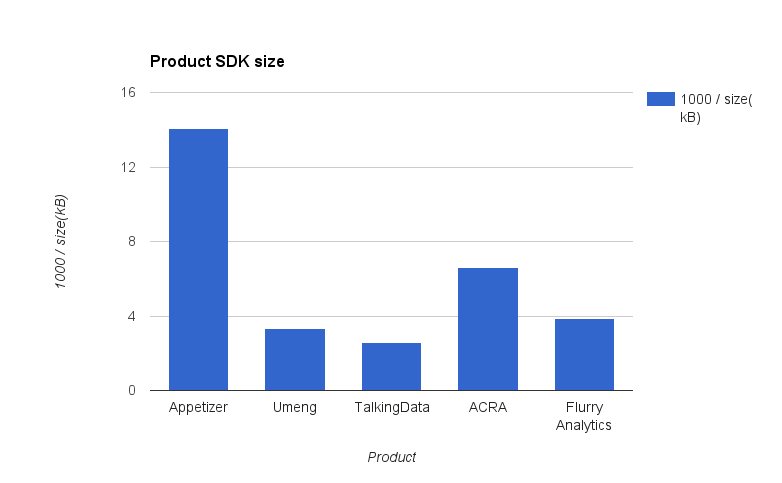
\includegraphics[width=1.0\textwidth]{SDK_size.png}
	\bicaption[fig:SDK_size]{这里将出现在插图索引中}{产品SDK占用空间}{Fig}{Product SDK size}
\end{figure}

\section{性能测试}
\label{sec:perfor_test}

性能测试部分主要计算Appetizer客户端SDK各个功能对原本的Android应用程序造成的额外开销,测试在不同设备不同系统上对比,测试在一个专门为测试编写的Appetizer Test App上进行。相关的测试设备信息如表\ref{tab:SDK_test_device}所示。

\begin{table}[!hpb]
	\centering
	\bicaption[tab:SDK_test_device]{指向一个表格的表目录索引}{测试设备列表}{Table}{Test device list}
	\begin{tabular}{c c c c c c} \toprule
		& System version & ROM & Chipset \\ \midrule
		Nexus 5 (Device A) & 4.4.2 & CyanogenMod 11 & Qualcomm Snapdragon 800 \\
		Nexus 5 (Device B) & 6.0.0 & Google ROM & Qualcomm Snapdragon 800 \\
		XiaoMi 4 & 6.0.1 & MIUI 7.3.2.0  & Qualcomm Snapdragon 801 \\
		Samsung Galaxy Note 4 & 5.1.1 & Samsung ROM & Qualcomm Snapdragon 805 \\
		HUAWEI Ascend Mate7 & 4.4.2 & EMUI 3.0 & HiSilicon Kirin 925 \\
		OPPO R7s & 4.4.4 & ColorOS 2.1 & Qualcomm Snapdragon 615 \\ \bottomrule
	\end{tabular}
\end{table}

其中Nexus 5有两部,分别运行Google官方ROM的Android 6.0.0和CyanogenMod 11,其他4部设备分别是小米4,三星Galaxy Note4,华为Ascend Mate 7和OPPO R7s,都是几大Android手机厂商2015年到2016年之间在中国市场使用量较大的主流设备,这些设备对于Appetizer客户端SDK的测试具有代表性。

所有测试数据根据设备状况不同都会在一定区间内浮动,本节的数据取得是多次测试结果的平均值。

\subsection{初始化开销}
\label{subsec:init_cost}

Appetizer客户端SDK需要被集成的Android应用程序在启动时,调用Application类的onCreate方法的时候调用Appetizer的初始化方法,该初始化方法是Appetizer客户端SDK开启所有功能必须执行的操作,该方法的开销直接影响到所有集成了Appetizer客户端SDK的Android应用程序的启动耗时。

\begin{figure}[!htp]
	\centering
	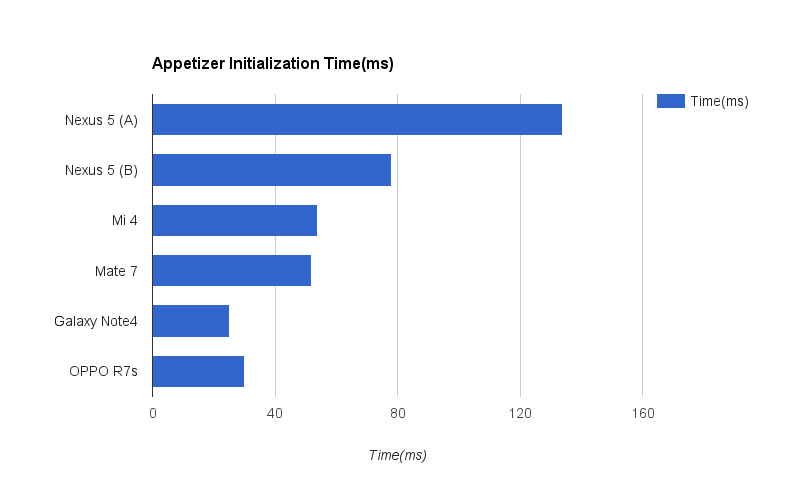
\includegraphics[width=1.0\textwidth]{init_time.png}
	\bicaption[fig:init_time]{这里将出现在插图索引中}{Appetizer初始化时间}{Fig}{Appetizer intialization time}
\end{figure}

因为Appetizer初始化的速度也就是程序运行的速度,和各种软件、硬件相关,从表\ref{fig:init_time}中难以得到Appetizer初始化开销和某一类因素的相关性,但可以看出Appetizer初始化开销在主流设备和较新的Android系统上都不大于100毫秒,对程序启动时间的影响不大。

\subsection{用户会话开销}
\label{subsec:session_cost}

用户会话主要在两种情况下存在开销,一种在用户切换页面的时候对会话信息的临时更新(保证崩溃可恢复),另一种是在用户结束会话的时候对完整会话的持久化存储。第二种情况通常在应用长时间运行在后台或者退出的时候发生,不会影响用户体验,因此只对第一种情况进行性能测试。

如表\ref{tab:SDK_session_time}所示是Android应用程序切换界面时,Appetizer用户会话更新一次的时间开销,所有测试设备的时间均在10毫秒以内,可以认为Appetizer客户端SDK用户会话收集功能在Android应用程序中产生的额外开销,对用户体验不会造成影响。

\begin{table}[!hpb]
	\centering
	\bicaption[tab:SDK_session_time]{指向一个表格的表目录索引}{Appetizer用户会话更新时间}{Table}{Appetizer app session update time}
	\begin{tabular}{c c c c c c} \toprule
		& Session update time (ms) \\ \midrule
		Nexus 5 (Device A) & 3ms$\sim$9ms \\
		Nexus 5 (Device B) & 1ms$\sim$4ms \\
		XiaoMi 4 & 1ms$\sim$4ms \\
		Samsung Galaxy Note 4 & 1ms$\sim$6ms \\
		HUAWEI Ascend Mate7 & 1ms$\sim$4ms \\
		OPPO R7s & 1ms$\sim$2ms \\ \bottomrule
	\end{tabular}
\end{table}


\subsection{ANR侦测开销}
\label{subsec:anr_cost}

\begin{table}[!hpb]
	\centering
	\bicaption[tab:SDK_ANR_time]{指向一个表格的表目录索引}{Appetizer ANR侦测主线程开销}{Table}{Appetizer ANR detector main thread cost}
	\begin{tabular}{c c c c c c} \toprule
		& ANR Runnable time (ms) \\ \midrule
		Nexus 5 (Device A) & 1ms$\sim$2ms \\
		Nexus 5 (Device B) & 1ms$\sim$2ms \\
		XiaoMi 4 & 1ms \\
		Samsung Galaxy Note 4 & 1ms$\sim$2ms \\
		HUAWEI Ascend Mate7 & 1ms \\
		OPPO R7s & 1ms$\sim$2ms \\ \bottomrule
	\end{tabular}
\end{table}

Appetizer的Android应用程序未响应(ANR)侦测功能,由一个ANR侦测线程每隔5秒发送Runnable到主线程(UI线程)执行一段程序,因此在Android应用程序在前台运行时ANR侦测发送到主线程执行的程序运行频率较高,而且是在UI线程执行,如果占用时间过长会让用户感到卡顿,因此在各个设备上对ANR侦测的开销进行测试。

测试结果如表\ref{tab:SDK_ANR_time}所示,测试结果为数十次测试得到时间开销的平均值,不包含主线程对Runnable调度的开销。从结果可以看出ANR侦测Runnable的运行开销不超过2毫秒,因此ANR侦测对Android应用程序的额外开销可以忽略不计。

\section{本章小节}

本章内容主要介绍了Appetizer客户端SDK和同类产品的功能对比,以及自身性能和开销的测试。

\ref{sec:functions}节对比了Appetizer同类产品友盟(Umeng)、TalkingData、雅虎公司的Flurry Analytics和腾讯公司的Bugly功能上的差异,展现了Appetizer客户端SDK在信息收集上覆盖了同类产品所没有的部分。

\ref{sec:SDK_size_compare}节对比了Appetizer客户端SDK和同类产品SDK之间空间占用大小,Appetizer客户端SDK在Android设备信息收集SDK中拥有占用空间最小的优势。

\ref{sec:perfor_test}节对Appetizer客户端SDK的性能开销在不同系统和不同主流Android设备上进行了测试。\ref{subsec:init_cost}小节对Appetizer客户端初始化的开销进行了测试,主流Android设备在Appetizer客户端SDK初始化阶段耗时都低于100毫秒,对用户体验影响不大。\ref{subsec:session_cost}小节对Appetizer客户端SDK的用户会话更新功能进行了开销测试,该事件会在用户切换Android应用界面时发生,在主流Android设备上该功能的耗时都低于10毫秒,对用户体验没有影响。\ref{subsec:anr_cost}小节对Appetizer客户端SDK的应用程序未响应(ANR)功能开销进行了测试,得到结果每隔5秒执行的功能额外开销对主线程的占用时间,在主流Android设备上不超过2毫秒,不会影响用户体验。
